\chapter{Author Extraction Example}\label{app:cha-author-extraction-example}

\section{Factor Product}\label{app:sec-factor-product}
\begin{table}[H]
\centering
$\Psi(LN_1,F\rs N_2,EC_2)$\par
\smallskip
\begin{tabular}{c c c l}
 \toprule
 $LN_1$ & $LN_2$ & $EC_2$ & \multicolumn{1}{c}{Value} \\
 \midrule
 $\mathit{false}$ & $\mathit{false}$ & $\mathit{false}$ & $(10\cdot10)\cdot\hphantom{0}1=100$\\
 $\mathit{false}$ & $\mathit{false}$ & $\mathit{true}$  & $(20\cdot\hphantom{0}1)\cdot\hphantom{0}1=20$\\
 $\mathit{false}$ & $\mathit{true}$  & $\mathit{false}$ & $(10\cdot10)\cdot30=\num{3000}$\\
 $\mathit{false}$ & $\mathit{true}$  & $\mathit{true}$  & $(20\cdot20)\cdot30=\num{12000}$\\
 $\mathit{true}$  & $\mathit{false}$ & $\mathit{false}$ & $(10\cdot10)\cdot10=\num{1000}$\\
 $\mathit{true}$  & $\mathit{false}$ & $\mathit{true}$  & $(\hphantom{0}1\cdot\hphantom{0}1)\cdot10=10$\\
 $\mathit{true}$  & $\mathit{true}$  & $\mathit{false}$ & $(10\cdot10)\cdot\hphantom{0}1=100$\\
 $\mathit{true}$  & $\mathit{true}$  & $\mathit{true}$  & $(\hphantom{0}1\cdot20)\cdot\hphantom{0}1=20$\\
 \bottomrule
\end{tabular}
\caption{Results of the \gls{factor product} $(\Psi(LN_1,EC_2)\times\Psi(LN_2,EC_2))\times\Psi(LN_1,LN_2)$ of the \glspl{factor} in \Cref{tab:example-factors}. For an exemplary calculation see \Cref{app:subsec-gd-example-calculation}.}
\label{tab:example-factor-product}
\end{table}
\section{Gibbs Distribution}\label{app:sec-gibbs-distribution}
\subsection{Exemplary Calculation}\label{app:subsec-gd-example-calculation}
The following calculation is based on \gls{factor graph} (a) in \Cref{fig:example-factor-graphs} with $\mathcal{X}=\{LN_1,LN_2,EC_2\}$.
It uses the \glspl{factor} defined in \Cref{tab:example-factors}.
\begin{subequations}
\begin{equation*}
\begin{split}
  \tilde{P}(LN_1{=}\mathit{true},LN_2{=}\mathit{false},EC_2{=}\mathit{false})&=\prod_{k=1}^{K}\Psi_k\left(\mathbf{D}_k\right) \\
  &=(\Psi(LN_1{=}\mathit{true},EC_2{=}\mathit{false})\\
  & \hspace{2em}\times\Psi(LN_2{=}\mathit{false},EC_2{=}\mathit{false}))\\
  & \hspace{2em}\times\Psi(LN_1{=}\mathit{true},LN_2{=}\mathit{false})\\
  &=(10\cdot10)\cdot10\\
  &=\num{1000}\\[1em]
\end{split}
\end{equation*}
\begin{equation*}
\begin{split}
  Z&=\sum_{EC_2,LN_2,LN_1}\tilde{P}\left(LN_1,LN_2,EC_2\right)\\
  &=\Psi(LN_1{=}\mathit{false},LN_2{=}\mathit{false},EC_2{=}\mathit{false})\\
  &\hspace{2em}+\Psi(LN_1{=}\mathit{false},LN_2{=}\mathit{false},EC_2{=}\mathit{true})\\
  &\hspace{2em}+\dots\\
  &\hspace{2em}+\Psi(LN_1{=}\mathit{true},LN_2{=}\mathit{true},EC_2{=}\mathit{true})\\
  &= \num{16250}\\[1em]
\end{split}
\end{equation*}
\begin{equation*}
\begin{split}
  P(LN_1{=}\mathit{true},LN_2{=}\mathit{false},EC_2{=}\mathit{false})&=\frac{1}{Z}\tilde{P}\left(LN_1{=}\mathit{true},LN_2{=}\mathit{false},EC_2{=}\mathit{false}\right) \\
  &=\frac{1}{\num{16250}}\cdot\num{1000}\\
  &\approx0.0615\\
\end{split}
\end{equation*}
\end{subequations}
\subsection{Full Distribution}\label{app:subsec-gd-full-distribution}
\begin{table}[H]
\centering
$P(LN_1,LN_2,EC_2)$\par
\smallskip
\begin{tabular}{c c c r}
 \toprule
 $LN_1$ & $LN_2$ & $EC_2$ & \multicolumn{1}{c}{Value} \\
 \midrule
 $\mathit{false}$ & $\mathit{false}$ & $\mathit{false}$ & $\num{100}/\num{16250}\approx0.0062$\\
 $\mathit{false}$ & $\mathit{false}$ & $\mathit{true}$  & $\num{20}/\num{16250}\approx0.0012$\\
 $\mathit{false}$ & $\mathit{true}$  & $\mathit{false}$ & $\num{3000}/\num{16250}\approx0.1846$\\
 $\mathit{false}$ & $\mathit{true}$  & $\mathit{true}$  & $\num{12000}/\num{16250}\approx0.7385$\\
 $\mathit{true}$  & $\mathit{false}$ & $\mathit{false}$ & $\num{1000}/\num{16250}\approx0.0615$\\
 $\mathit{true}$  & $\mathit{false}$ & $\mathit{true}$  & $\num{10}/\num{16250}\approx0.0006$\\
 $\mathit{true}$  & $\mathit{true}$  & $\mathit{false}$ & $\num{100}/\num{16250}\approx0.0062$\\
 $\mathit{true}$  & $\mathit{true}$  & $\mathit{true}$  & $\num{20}/\num{16250}\approx0.0012$\\
 \bottomrule
\end{tabular}
\caption{Values of the \Gls{gibbs distribution} $P(LN_1,LN_2,EC_2)$ using the two \glspl{factor} in \Cref{tab:example-factors}.}
\label{tab:example-factor-product}
\end{table}
\section{Conditional Random Fields}\label{app:sec-conditional-random-fields}
\subsection{Calculation of Factor With $\mathbf{D}\subseteq\mathbf{X}$}\label{app:subsec-gd-example-calculation}
With the following calculation we demonstrate that a \gls{factor} $\Psi(\mathbf{D})$ with $\mathbf{D}\subseteq\mathbf{X}$ cancels out during the calculation of $P(\mathbf{Y}|\mathbf{X})$.
For this we consider two factors, $\Psi(LN_1,EC_1)$ and $\Psi(EC_1,EC_2)$.
The resulting \gls{factor graph} is shown in \Cref{fig:example-x-only-factor-graph}.
\begin{figure}[H]
\centering
\newcommand{\factorgraphnodes}{%
  \node[latent] (ln) {$LN_1$}; %
  \node[obs, below=1.8cm of ln] (ec1) {$EC_1$}; %
  \node[obs, right=2.4cm of ec1] (ec2) {$EC_2$}; %
}
\begin{tikzpicture}
  \factorgraphnodes

  \factor[above=0.8cm of ec1] {ec1-ln-f} {right:$\Psi(LN_1,EC_1)$} {} {}; %
  \factor[right=1.1cm of ec1] {ec1-ec2-f} {above:$\Psi(EC_1,EC_2)$} {} {}; %
  \edge[-] {ln} {ec1};
  \edge[-] {ec1} {ec2};
\end{tikzpicture}

\caption{%
  Factor graph containing two factors where $\Psi(EC_1,EC_2)$ only contains \glspl{observed variable}.
}
\label{fig:example-x-only-factor-graph}
\end{figure}
Based on the definition of \glspl{crf} in \Cref{equ:crf-factor} we have for example:
\begin{equation*}
\begin{split}
  &P(LN_1{=}\mathit{true},EC_1{=}\mathit{true}\mid EC_2{=}\mathit{false})\\
  &\hspace{2em}=\frac{1}{Z(EC_1{=}\mathit{true},EC_2{=}\mathit{false})}\cdot\tilde{P}\left(LN_1{=}\mathit{true},EC_1{=}\mathit{true},EC_2{=}\mathit{false}\right)\\[0.25cm]
  &\hspace{2em}=\frac{\tilde{P}\left(LN_1{=}\mathit{true},EC_1{=}\mathit{true},EC_2{=}\mathit{false}\right)}{\splitfrac{\tilde{P}(LN_1{=}\mathit{false},EC_1{=}\mathit{true},EC_2{=}\mathit{false})}
    {+\tilde{P}(LN_1{=}\mathit{true},EC_1{=}\mathit{true},EC_2{=}\mathit{false})}}\\[0.25cm]
  &\hspace{2em}=\frac{\Psi(LN_1{=}\mathit{true},EC_1{=}\mathit{false})\times\Psi(EC_1{=}\mathit{true},EC_2{=}\mathit{false})}{\splitfrac{\Psi(LN_1{=}\mathit{true},EC_1{=}\mathit{false})\times\Psi(EC_1{=}\mathit{true},EC_2{=}\mathit{false})}
  {+\Psi(LN_1{=}\mathit{true},EC_1{=}\mathit{true})\times\Psi(EC_1{=}\mathit{true},EC_2{=}\mathit{false})}}\\[0.25cm]
  &\hspace{2em}=\frac{\Psi(EC_1{=}\mathit{true},EC_2{=}\mathit{false})\times\Psi(LN_1{=}\mathit{true},EC_1{=}\mathit{false})}{\splitfrac{\Psi(EC_1{=}\mathit{true},EC_2{=}\mathit{false})\times(\Psi(LN_1{=}\mathit{true},EC_1{=}\mathit{false})}
  {+\Psi(LN_1{=}\mathit{true},EC_1{=}\mathit{true}))}}\\[0.25cm]
  &\hspace{2em}=\frac{\Psi(LN_1{=}\mathit{true},EC_1{=}\mathit{false})}{\Psi(LN_1{=}\mathit{true},EC_1{=}\mathit{false})+\Psi(LN_1{=}\mathit{true},EC_1{=}\mathit{true})}\\[0.25cm]
  &\hspace{2em}=\frac{\tilde{P}\left(LN_1{=}\mathit{true},EC_1{=}\mathit{true}\right)}{\tilde{P}(LN_1{=}\mathit{false},EC_1{=}\mathit{true})+\tilde{P}(LN_1{=}\mathit{true},EC_1{=}\mathit{true})}\\[0.25cm]
  &\hspace{2em}={P}\left(LN_1{=}\mathit{true}\mid EC_1{=}\mathit{true}\right).\\
\end{split}
\end{equation*}

Thereby, the distributive property allows us to factor out $\Psi(EC_1{=}\mathit{true},EC_2{=}\mathit{false})$ in the denominator which allows us to completely remove this \gls{factor} from the equation.
This example demonstrates that a \gls{factor} with $\mathbf{D}\subseteq\mathbf{X}$ does not have an impact on the result of $P(\mathbf{Y}|\mathbf{X})$.

\subsection{Exemplary Calculation}\label{app:subsec-crf-example-calculation}
The following calculation is based on \gls{factor graph} (a) in \Cref{fig:example-factor-graphs} with $\mathbf{X}=\{EC_2\}$ and $\mathbf{Y}=\{LN_1,LN_2\}$.
It uses the \glspl{factor} defined in \Cref{tab:example-factors}.

\begin{subequations}
\begin{equation*}
\begin{split}
  \tilde{P}(LN_1{=}\mathit{true},LN_2{=}\mathit{false},EC_2{=}\mathit{false})&=\prod_{k=1}^{K}\Psi_k\left(\mathbf{D}_k\right) \\
  &=(\Psi(LN_1{=}\mathit{true},EC_2{=}\mathit{false})\\
  &\hspace{2em}\times\Psi(LN_2{=}\mathit{false},EC_2{=}\mathit{false}))\\
  &\hspace{2em}\times\Psi(LN_1{=}\mathit{true},LN_2{=}\mathit{false})\\
  &=(10\cdot10)\cdot10\\
  &=\num{1000}\\[1em]
\end{split}
\end{equation*}
\begin{equation*}
\begin{split}
  Z(EC_2{=}\mathit{false})&=\sum_{LN_2}\tilde{P}\left(LN_1,LN_2,EC_2{=}\mathit{false}\right)\\
  &=\tilde{P}(LN_1{=}\mathit{false},LN_2{=}\mathit{false},EC_2{=}\mathit{false})\\
  &\hspace{2em}+\tilde{P}(LN_1{=}\mathit{false},LN_2{=}\mathit{true},EC_2{=}\mathit{false})\\
  &\hspace{2em}+\tilde{P}(LN_1{=}\mathit{true},LN_2{=}\mathit{false},EC_2{=}\mathit{false})\\
  &\hspace{2em}+\tilde{P}(LN_1{=}\mathit{true},LN_2{=}\mathit{true},EC_2{=}\mathit{false})\\
  &=100+\num{3000}+\num{1000}+100\\
  &=\num{4200}\\[1em]
\end{split}
\end{equation*}
\begin{equation*}
\begin{split}
  &P(LN_1{=}\mathit{true},LN_2{=}\mathit{false}\mid EC_2{=}\mathit{false})\\
  &\hspace{2em}=\frac{1}{Z(EC_2{=}\mathit{false})}\cdot\tilde{P}\left(LN_1{=}\mathit{true},LN_2{=}\mathit{false},EC_2{=}\mathit{false}\right)\\
  &\hspace{2em}=\frac{1}{\num{4200}}\cdot\num{1000}\\
  &\hspace{2em}\approx0.2381\\
\end{split}
\end{equation*}
\end{subequations}
\section{Linear-Chain CRFs}\label{app:sec-linear-chain-crfs}
\subsection{Additional Factors}\label{app:subsec-lccrf-additional-factors}

\begin{table}[H]
\begin{minipage}{0.5\linewidth}
\centering
$\Psi(\texttt{start},LN_1)$\par
\smallskip
\begin{tabular}{c c c}
 \toprule
 \texttt{start} & $LN_1$ & Value \\
 \midrule
 $\mathit{false}$ & $\mathit{false}$ & $1$ \\
 $\mathit{false}$ & $\mathit{true}$ & $1$ \\
 $\mathit{true}$ & $\mathit{false}$ & $30$ \\
 $\mathit{true}$ & $\mathit{true}$ & $10$ \\
 \bottomrule
\end{tabular}
\end{minipage}
\hfill
\begin{minipage}{0.5\linewidth}
\centering
$\Psi(LN_1,EC_1)$\par
\smallskip
\begin{tabular}{c c c}
 \toprule
 $LN_1$ & $EC_1$ & Value \\
 \midrule
 $\mathit{false}$ & $\mathit{false}$ & $30$ \\
 $\mathit{false}$ & $\mathit{true}$ & $1$ \\
 $\mathit{true}$ & $\mathit{false}$ & $1$ \\
 $\mathit{true}$ & $\mathit{true}$ & $10$ \\
 \bottomrule
\end{tabular}
\end{minipage}
\caption{Two additional factors for the author extraction example in \Cref{fig:example-linear-chain-crf}}
\label{tab:example-linear-chain-crf-factors}
\end{table}

\subsection{Additional Energy Functions}\label{app:subsec-lccrf-additional-energy-functions}
\begin{table}[H]
\begin{minipage}{0.5\linewidth}
\centering
$\Psi(\texttt{start},LN_1)$\par
\smallskip
\begin{tabular}{c c c}
 \toprule
 \texttt{start} & $LN_1$ & Value \\
 \midrule
 $\mathit{false}$ & $\mathit{false}$ & $-\ln(1) = 0\hphantom{.00001}$ \\
 $\mathit{false}$ & $\mathit{true}$ & $-\ln(1) = 0\hphantom{.00001}$ \\
 $\mathit{true}$ & $\mathit{false}$ & $-\ln(30)\approx-3.4012$ \\
 $\mathit{true}$ & $\mathit{true}$ & $-\ln(10)\approx-2.3026$ \\
 \bottomrule
\end{tabular}
\end{minipage}
\hfill
\begin{minipage}{0.5\linewidth}
\centering
$\Psi(LN_1,EC_1)$\par
\smallskip
\begin{tabular}{c c c}
 \toprule
 $LN_1$ & $EC_1$ & Value \\
 \midrule
 $\mathit{false}$ & $\mathit{false}$ & $-\ln(30)\approx-3.4012$ \\
 $\mathit{false}$ & $\mathit{true}$ & $-\ln(1) = 0\hphantom{.00001}$ \\
 $\mathit{true}$ & $\mathit{false}$ & $-\ln(1) = 0\hphantom{.00001}$ \\
 $\mathit{true}$ & $\mathit{true}$ & $-\ln(10)\approx-2.3026$ \\
 \bottomrule
\end{tabular}
\end{minipage}
\caption{\Glspl{energy function} for the additional \glspl{factor} in \Cref{tab:example-linear-chain-crf-factors}.}
\label{tab:example-linear-chain-crf-energy-functions}
\end{table}

\subsection{Feature Functions}\label{app:subsec-lccrf-feature-functions}

\begin{table}[H]
\centering
\begin{tabular}{c l c}
 \toprule
 Index & \multicolumn{1}{c}{Feature function $f_k$} & Weight $\theta_k$ \\
 \midrule
 $k=1$ & $\identityfun\left\{LN_1{=}\mathit{false},\texttt{start}{=}\mathit{true}\right\}$ & $-\ln(30)\approx-3.4012$ \\
 $k=2$ & $\identityfun\left\{LN_1{=}\mathit{true},\texttt{start}{=}\mathit{true}\right\}$ & $-\ln(10)\approx-2.3026$ \\
 $k=3$ & $\identityfun\left\{LN_2{=}\mathit{false},\ \ \ \ \hspace{-0.1mm}LN_1{=}\mathit{true}\right\}$ & $-\ln(10)\approx-2.3026$\\
 $k=4$ & $\identityfun\left\{LN_2{=}\mathit{true},\ \ \ \ \hspace{0.4mm}LN_1{=}\mathit{false}\right\}$ & $-\ln(30)\approx-3.4012$ \\
 \bottomrule
\end{tabular}
\caption{\Glspl{feature function} $\tilde{f}_k(Y_n,Y_{n-1})$ representing $\Psi(\texttt{start},LN_1)$ and $\Psi(LN_1,LN_2)$. Note the inverted argument order of $\tilde{f}_k$.}
\label{tab:example-linear-chain-crf-feature-functions-f-k}
\end{table}

\begin{table}[H]
\centering
\begin{tabular}{c l c}
 \toprule
 Index & \multicolumn{1}{c}{Feature function $f_l$ } & Weight $\theta_l$ \\
 \midrule
 $l=1$ & $\identityfun\left\{LN_1{=}\mathit{false},EC_1{=}\mathit{false}\right\}$ & $-\ln(30)\approx-3.4012$ \\
 $l=2$ & $\identityfun\left\{LN_1{=}\mathit{true},\hspace{0.4mm}EC_1{=}\mathit{true}\right\}$ & $-\ln(10)\approx-2.3026$ \\
 $l=3$ & $\identityfun\left\{LN_2{=}\mathit{false},EC_2{=}\mathit{false}\right\}$ & $-\ln(10)\approx-2.3026$ \\
 $l=4$ & $\identityfun\left\{LN_2{=}\mathit{true},EC_2{=}\mathit{false}\right\}$ & $-\ln(10)\approx-2.3026$ \\
 $l=5$ & $\identityfun\left\{LN_2{=}\mathit{true},EC_2{=}\mathit{true}\right\}$ & $-\ln(20)\approx-2.9957$ \\
 \bottomrule
\end{tabular}
\caption{\Glspl{feature function} $\tilde{f}_l(Y_n,\tilde{\mathbf{X}}_n)$ representing $\Psi(LN_1,EC_1)$ and $\Psi(LN_2,EC_2)$. Note the inverted argument order of $\tilde{f}_l$.}
\label{tab:example-linear-chain-crf-feature-functions-f-l}
\end{table}

\newpage

\subsection{Exemplary Calculation}\label{app:subsec-lccrf-example-calculation}
The following calculation is based on the \gls{linear-chain crf} from \Cref{fig:example-linear-chain-crf} with $\mathbf{X}=\{EC_1,EC_2\}$ and $\mathbf{Y}=\{\texttt{start},LN_1,LN_2\}$.
It uses the \glspl{feature function} defined in \Cref{app:subsec-lccrf-feature-functions}.
The \glspl{assignment} are based on the second reference string in \Cref{fig:example-reference-strings}.

\begin{subequations}
\begin{equation*}
\begin{split}
  &\tilde{P}(\texttt{start}{=}\mathit{true},LN_1{=}\mathit{true},LN_2{=}\mathit{false},EC_1{=}\mathit{true},EC_2{=}\mathit{false})\\
  &\hspace{2em} = \exp\left\{ -\sum_{n=1}^N \left(\sum_{k=1}^K\theta_k \tilde{f}_k\left(\vphantom{\tilde{X}}Y_n,Y_{n-1}\right)+\sum_{l=1}^L\theta_l \tilde{f}_l\left(Y_n,\mathbf{\tilde{X}}_n\right)\right) \right\} \\
  &\hspace{2em} = \exp\Big\{-\Big(\theta_{k=1}f_{k=1}(LN_1{=}\mathit{true},\texttt{start}{=}\mathit{true})\\
  &\hspace{6em}\vphantom{\Big\{}+\cdots+\theta_{k=4}f_{k=4}(LN_1{=}\mathit{true},\texttt{start}{=}\mathit{true})\\
  &\hspace{4em}\vphantom{\Big\{}+\theta_{l=1}f_{l=1}(LN_1{=}\mathit{true},EC_1{=}\mathit{true})\\
  &\hspace{6em}\vphantom{\Big\{}+\cdots+\theta_{l=5}f_{l=5}(LN_1{=}\mathit{true},EC_1{=}\mathit{true})\\
  &\hspace{4em}\vphantom{\Big\{}+\theta_{k=1}f_{k=1}(LN_2{=}\mathit{false},LN_1{=}\mathit{true})\\
  &\hspace{6em}\vphantom{\Big\{}+\cdots+\theta_{k=4}f_{k=4}(LN_2{=}\mathit{false},LN_1{=}\mathit{true}) \\
  &\hspace{4em}\vphantom{\Big\{}+\theta_{l=1}f_{l=1}(LN_2{=}\mathit{false},EC_2{=}\mathit{false})\\
  &\hspace{6em}\vphantom{\Big\{}+\cdots+\theta_{l=5}f_{l=5}(LN_2{=}\mathit{false},EC_2{=}\mathit{false})\Big)\Big\}\\
  &\hspace{2em} = \exp\Big\{-\Big(-\log(30)\cdot0-\log(10)\cdot1-\log(10)\cdot0-\log(30)\cdot0\\
  &\hspace{4em}\vphantom{\Big\{}-\log(30)\cdot0-\log(10)\cdot1-\log(10)\cdot0-\log(10)\cdot0-\log(20)\cdot0\\
  &\hspace{4em}\vphantom{\Big\{}-\log(30)\cdot0-\log(10)\cdot0-\log(10)\cdot1-\log(30)\cdot0\\
  &\hspace{4em}\vphantom{\Big\{}-\log(30)\cdot0-\log(10)\cdot0-\log(10)\cdot1-\log(10)\cdot0-\log(20)\cdot0\Big)\Big\}\\
  &\hspace{2em}=\exp\Big\{-\Big(-\log(10)-\log(10)-\log(10)-\log(10)\Big)\Big\}\\
  &\hspace{2em}=\exp\Big\{4\cdot\log(10)\Big\}\\
  &\hspace{2em}\vphantom{\Big\{}=\num{10000}\\[1em]
\end{split}
\end{equation*}
\begin{equation*}
\begin{split}
  &Z(EC_1{=}\mathit{true},EC_2{=}\mathit{false})\\
  &\hspace{2em}=\sum_{\texttt{start},LN_1,LN_2}\tilde{P}\left(\texttt{start},LN_1,LN_2,EC_1{=}\mathit{true},EC_2{=}\mathit{false}\right)\\
  &\hspace{2em}=\tilde{P}(\texttt{start}{=}\mathit{false},LN_1{=}\mathit{false},LN_2{=}\mathit{false},EC_1{=}\mathit{true},EC_2{=}\mathit{false})\\
  &\hspace{4em}+\tilde{P}(\texttt{start}{=}\mathit{false},LN_1{=}\mathit{false},LN_2{=}\mathit{true},EC_1{=}\mathit{true},EC_2{=}\mathit{false})\\
  &\hspace{4em}+\tilde{P}(\texttt{start}{=}\mathit{false},LN_1{=}\mathit{true},LN_2{=}\mathit{false},EC_1{=}\mathit{true},EC_2{=}\mathit{false})\\
  &\hspace{4em}+\tilde{P}(\texttt{start}{=}\mathit{false},LN_1{=}\mathit{true},LN_2{=}\mathit{true},EC_1{=}\mathit{true},EC_2{=}\mathit{false})\\
  &\hspace{4em}+\tilde{P}(\texttt{start}{=}\mathit{true},LN_1{=}\mathit{false},LN_2{=}\mathit{false},EC_1{=}\mathit{true},EC_2{=}\mathit{false})\\
  &\hspace{4em}+\tilde{P}(\texttt{start}{=}\mathit{true},LN_1{=}\mathit{false},LN_2{=}\mathit{true},EC_1{=}\mathit{true},EC_2{=}\mathit{false})\\
  &\hspace{4em}+\tilde{P}(\texttt{start}{=}\mathit{true},LN_1{=}\mathit{true},LN_2{=}\mathit{false},EC_1{=}\mathit{true},EC_2{=}\mathit{false})\\
  &\hspace{4em}+\tilde{P}(\texttt{start}{=}\mathit{true},LN_1{=}\mathit{true},LN_2{=}\mathit{true},EC_1{=}\mathit{true},EC_2{=}\mathit{false})\\
  %start  LN_1   LN_2  Result
  %  F     F      F    1    1    30    10   10
  %  F     F      T    1    1    1     10   300
  %  F     T      F    1    10   1     10   1000
  %  F     T      T    1    10   10    10   100
  %  T     F      F    30   1    30    10   3000
  %  T     F      T    30   1    10    10   9000
  %  T     T      F    10   10   1     10   10000
  %  T     T      T    10   10   10    10   1000
  &\hspace{2em}=10+300+\num{1000}+100+\num{3000}+\num{9000}+\num{10000}+\num{1000}\\
  &\hspace{2em}=\num{24410}\\[1em]
\end{split}
\end{equation*}
\begin{equation*}
\begin{split}
  &P(\texttt{start}{=}\mathit{true},LN_1{=}\mathit{true},LN_2{=}\mathit{false}\mid EC_1{=}\mathit{true},EC_2{=}\mathit{false})\\
  &\hspace{2em}=\frac{1}{Z(EC_1{=}\mathit{true},EC_2{=}\mathit{false})}\\
  &\hspace{4em}\cdot\tilde{P}\left(\texttt{start}{=}\mathit{true},LN_1{=}\mathit{true},LN_2{=}\mathit{false},EC_1{=}\mathit{true},EC_2{=}\mathit{false}\right)\\
  &\hspace{2em}=\frac{1}{\num{24410}}\cdot\num{10000}\\
  &\hspace{2em}\approx0.41\\
\end{split}
\end{equation*}
\end{subequations}

\newpage

\section{Log-Likelihood Function}\label{app:sec-log-likelihood-function}
The following calculation is based on \gls{factor graph} in \Cref{fig:example-linear-chain-crf} that represents a \gls{linear-chain crf} with $\mathbf{X}=\{EC_1,EC_2\}$ and $\mathbf{Y}=\{\texttt{start},LN_1,LN_2\}$.
It uses the \glspl{feature function} and corresponding weights from \Cref{app:subsec-lccrf-feature-functions}.
Further, we have $\mathcal{D}=\{\mathpzc{d}^{(1)},\dots,\mathpzc{d}^{(4)}\}$ consisting of the four reference strings in \Cref{fig:example-reference-strings}.
Based on this, we have the following log-likelihood function:
\begin{equation*}
  \begin{split}
    \ell\left(\bm{\tilde{\theta}}:\mathcal{D}\right) = & \sum_{m=1}^M \left(-\sum_{n=1}^N \left(\sum_{k=1}^K\theta_k \tilde{f}_k\left(Y_n^{(m)},Y_{n-1}^{(m)}\right)+\sum_{l=1}^L\theta_l \tilde{f}_l\left(Y_n^{(m)},\mathbf{\tilde{X}}_n^{(m)}\right)\right)\right. \\
    &\left.-\log Z\left(\mathbf{X}^{(m)}\right)\vphantom{\sum_{l=1}^L}\right)\\
    =&-\sum_{n=1}^N \left(\sum_{k=1}^K\theta_k \tilde{f}_k\left(Y_n^{(1)},Y_{n-1}^{(1)}\right)+\sum_{l=1}^L\theta_l \tilde{f}_l\left(Y_n^{(1)},\mathbf{\tilde{X}}_n^{(1)}\right)\right)-\log Z\left(\mathbf{X}^{(1)}\right)\vphantom{\sum_{l=1}^L}\\
    &+\cdots\\
    &+-\sum_{n=1}^N \left(\sum_{k=1}^K\theta_k \tilde{f}_k\left(Y_n^{(4)},Y_{n-1}^{(4)}\right)+\sum_{l=1}^L\theta_l \tilde{f}_l\left(Y_n^{(4)},\mathbf{\tilde{X}}_n^{(4)}\right)\right)-\log Z\left(\mathbf{X}^{(4)}\right)\vphantom{\sum_{l=1}^L}\\
    =&\Big(\log(30)+\log(30)+\log(30)+\log(10)\Big)-\log\left(\num{370510}\right)\\
    &\Big(\log(10)+\log(10)+\log(10)+\log(10)\Big)-\log\left(\num{24410}\right)\\
    &\Big(\log(30)+\log(30)+\log(30)+\log(20)\Big)-\log\left(\num{567360}\right)\\
    &\Big(\log(30)+\log(30)+\log(30)+\log(20)\Big)-\log\left(\num{567360}\right)\\
    \approx&12.5062-12.8226\\
    &+9.2103-10.1027\\
    &+13.1993-13.2487\\
    &+13.1993-13.2487\\
    \approx&-1.3076
 \end{split}
\end{equation*}
Note that, for the second reference string $\mathpzc{d}^{(2)}$, we calculate the values of the unnormalized measure
\begin{equation*}
  \tilde{P}(\mathbf{Y}^{(2)}\mid\mathbf{X}^{(2)})=-\sum_{n=1}^N \left(\sum_{k=1}^K\theta_k \tilde{f}_k\left(Y_n^{(2)},Y_{n-1}^{(2)}\right)+\sum_{l=1}^L\theta_l \tilde{f}_l\left(Y_n^{(2)},\mathbf{\tilde{X}}_n^{(2)}\right)\right)
\end{equation*}
and the corresponding normalizing constant
\begin{equation*}
Z\left(\mathbf{X}^{(2)}\right)
\end{equation*}
in \Cref{app:subsec-lccrf-example-calculation}.

% Z(X) calculations
% Z(X^1): EC_1=F, EC_2=F
% Z(X^2): EC_1=T, EC_2=F
% Z(X^3): EC_1=F, EC_2=T
% Z(X^4): EC_1=F, EC_2=T

% Z(EC_1=F,EC_2=T):
  %start  LN_1   FN_2    L1,s   L1,E1    F2,L1   F2,E2
  %  F     F      F      1      30       30      20   18000
  %  F     F      T      1      30       1       1    30
  %  F     T      F      1      1        1       20   20
  %  F     T      T      1      1        10      1    10
  %  T     F      F      30     30       30      20   540000
  %  T     F      T      30     30       10      1    9000
  %  T     T      F      10     1        1       20   200
  %  T     T      T      10     1        10      1    100

% Z(EC_1=F,EC_2=F):
  %start  LN_1   FN_2    L1,s   L1,E1    F2,L1   F2,E2
  %  F     F      F      1      30       30      10   9000
  %  F     F      T      1      30       1       10   300
  %  F     T      F      1      1        1       10   10
  %  F     T      T      1      1        10      10   100
  %  T     F      F      30     30       30      10   270000
  %  T     F      T      30     30       10      10   90000
  %  T     T      F      10     1        1       10   100
  %  T     T      T      10     1        10      10   1000

% 1: s=t, ln=f,fn=f,e1=f,e2=f
% 3: s=t, ln=f,fn=f,el=f,e2=t
\section{Distantly Supervised Training Sets}\label{app:sec-generalized-expectation}
\subsection{Author Name Matching}\label{app:author-name-matching}
\Cref{tab:example-author-list} contains an author list that we use for our author matching example.
\Cref{fig:example-goddag-1-final}, \Cref{fig:example-goddag-2-final}, and \Cref{fig:example-goddag-3-final} show the final \glspl{goddag} for the first three reference strings in \Cref{fig:example-reference-strings}, matched against the authors in \Cref{tab:example-author-list}.
\begin{table}[h]
\centering
\begin{tabular}{l l}
 \toprule
 First Names & Last Names\\
 \midrule
 Friedrich & M\"{u}ller\\
 Fritz & M\"{u}ller\\
 Max & M\"{u}ller\\
 Max & Wagner\\
 Max Friedrich & Schmidt\\
 Mia & Friedrich\\
 Mia & Wagner\\
 \bottomrule
\end{tabular}
\caption{Example author list for demonstrating the author matching.}
\label{tab:example-author-list}
\end{table}
\begin{figure}[h]
  \centering
%\hspace*{-1.25cm}
%\resizebox{\linewidth}{!}{%
  \begin{tikzpicture}
  \tikzset{ellipsenode/.style={ellipse,thick,draw}}
\tikzset{rectanglenode/.style={rectangle,draw}}
\tikzset{directededge/.style={->,> = latex,thick}}



  \node[rectanglenode] (l1)                       {Mia};
  \node[rectanglenode] (l2)  [right=of l1]        {Friedrich};
  \node[rectanglenode] (l3)  [right=of l2]        {(2010):};
  \node[rectanglenode] (l4)  [right=of l3]        {Title};
  \node                (l5)  [right=0.25cm of l4]        {\textbf{\dots}};
  \node[rectanglenode] (l6)  [right=0.25cm of l5]        {Springer.};
  \node[ellipsenode]   (fn1) [above=of l1]        {FN};
  \node[ellipsenode]   (ln1) [above=of l2]        {LN};
  \node[ellipsenode]   (o1)  [above=of l3]        {O};
  \node[ellipsenode]   (o2)  [above=of l4]        {O};
  \node[ellipsenode]   (o3)  [above=of l6]        {O};
  \node[ellipsenode]   (a1)  [above right=of fn1] {AU};
  \node[ellipsenode]   (r)   [above right=of a1]  {root};

  \foreach \from/\to in {r/a1,r/o1,r/o2,r/o2,r/o3,a1/fn1,a1/ln1,fn1/l1,ln1/l2,o1/l3,o2/l4,o3/l6}
  \draw[directededge] (\from) -- (\to);
\end{tikzpicture}


%}
\caption{Final \gls{goddag} for the first reference string in \Cref{fig:example-reference-strings}.}
\label{fig:example-goddag-1-final}
\end{figure}
\begin{figure}[h]
  \centering
%\hspace*{-1.25cm}
%\resizebox{\linewidth}{!}{%
  % Müller, Friedrich (2010): Title of the second example, Berlin: Springer.
\begin{tikzpicture}
  \tikzset{ellipsenode/.style={ellipse,thick,draw}}
\tikzset{rectanglenode/.style={rectangle,draw}}
\tikzset{directededge/.style={->,> = latex,thick}}



  \node[rectanglenode] (l1)                       {M\"{u}ller,};
  \node[rectanglenode] (l2)  [right=of l1]        {Friedrich};
  \node[rectanglenode] (l3)  [right=of l2]        {(2010):};
  \node[rectanglenode] (l4)  [right=of l3]        {Title};
  \node                (l5)  [right=0.25cm of l4]        {\textbf{\dots}};
  \node[rectanglenode] (l6)  [right=0.25cm of l5]        {Springer.};
  \node[ellipsenode]   (ln1) [above=of l1]        {LN};
  \node[ellipsenode]   (fn1) [above=of l2]        {FN};
  \node[ellipsenode]   (o1)  [above=of l3]        {O};
  \node[ellipsenode]   (o2)  [above=of l4]        {O};
  \node[ellipsenode]   (o3)  [above=of l6]        {O};
  \node[ellipsenode]   (a1)  [above right=of ln1] {AU};
  \node[ellipsenode]   (r)   [above right=of a1]  {root};

  \foreach \from/\to in {r/a1,r/o1,r/o2,r/o2,r/o3,a1/ln1,a1/fn1,ln1/l1,fn1/l2,o1/l3,o2/l4,o3/l6}
  \draw[directededge] (\from) -- (\to);
\end{tikzpicture}


%}
\caption{Final \gls{goddag} for the second reference string in \Cref{fig:example-reference-strings}.}
\label{fig:example-goddag-2-final}
\end{figure}
\begin{figure}[h]
  \centering
%\hspace*{-1.25cm}
%\resizebox{\linewidth}{!}{%
  % Fritz Müller, Fritz Schmidt (2010): Friedrich in title, Berlin: Springer.
\begin{tikzpicture}
  \tikzset{ellipsenode/.style={ellipse,thick,draw}}
\tikzset{rectanglenode/.style={rectangle,draw}}
\tikzset{directededge/.style={->,> = latex,thick}}



  \node[rectanglenode] (l1)                       {Fritz};
  \node[rectanglenode] (l2)  [right=of l1]        {M\"{u}ller,};
  \node[rectanglenode] (l3)  [right=of l2]        {Fritz};
  \node[rectanglenode] (l4)  [right=of l3]        {Schmidt};
  \node[rectanglenode] (l5)  [right=of l4]        {(2010):};
  \node                (l6)  [right=0.25cm of l5] {\textbf{\dots}};
  \node[rectanglenode] (l7)  [right=0.25cm of l6] {Springer.};
  \node[ellipsenode]   (fn1) [above=of l1]        {FN};
  \node[ellipsenode]   (ln1) [above=of l2]        {LN};
  \node[ellipsenode]   (fn2) [above=of l3]        {FN};
  \node[ellipsenode]   (o1)  [above=of l4]        {O};
  \node[ellipsenode]   (o2)  [above=of l5]        {O};
  \node[ellipsenode]   (o3)  [above=of l7]        {O};
  \node[ellipsenode]   (a1)  [above right=of fn1] {AU};
  \node[ellipsenode]   (a2)  [right=of a1]        {AU};
  \node[ellipsenode]   (r)   [above right=of a1]  {root};

  \foreach \from/\to in {r/a1,r/a2,r/o1,r/o2,r/o2,r/o3,a1/fn1,a1/ln1,a2/ln1,a2/fn2,fn1/l1,ln1/l2,fn2/l3,o1/l4,o2/l5,o3/l7}
  \draw[directededge] (\from) -- (\to);
\end{tikzpicture}


%}
\caption{Final \gls{goddag} for the third reference string in \Cref{fig:example-reference-strings}.}
\label{fig:example-goddag-3-final}
\end{figure}

\clearpage
\subsection{\glsentryshort{ge} Constraints}\label{app:subsec-ge-constraints}
\begin{table}[h]
\centering
\begin{tabular}{l l l l l l}
  \toprule
  Word &\multicolumn{1}{c}{\texttt{B-FN}}&\multicolumn{1}{c}{\texttt{B-LN}}&\multicolumn{1}{c}{\texttt{I-FN}}&\multicolumn{1}{c}{\texttt{I-LN}}&\multicolumn{1}{c}{\texttt{O}}\\
  \midrule    %    B-FN      I-FN               B-LN         I-LN                O
  (2010):     & $0/1=0$   & $0/1=0$          & $0/1=0$    & $0/1=0$          & $1/1=1$   \\
  Berlin      & $0/2=0$   & $0/2=0$          & $0/2=0$    & $0/2=0$          & $2/2=1$   \\
  Fourth      & $0/1=0$   & $0/1=0$          & $0/1=0$    & $0/1=0$          & $1/1=1$   \\
  Friedrich   & $0/4=0$   & $2/4=0.5$        & $0/4=0$    & $1/4=0.25$       & $1/4=0.25$\\
  Fritz       & $0/1=0$   & $0/1=0$          & $1/1=1$  & $0/1=0$          & $0/1=0$   \\
  Max         & $3/3=1$   & $0/3=0$          & $0/3=0$    & $0/3=0$          & $0/3=0$   \\
  Mia         & $2/2=1$   & $0/2=0$          & $0/2=0$    & $0/2=0$          & $0/2=0$   \\
  M\"{u}ller, & $0/3=0$   & $2/3\approx0.33$ & $0/3=0$    & $1/3\approx0.67$ & $0/3=0$   \\
  Schmidt     & $0/1=0$   & $0/1=0$          & $0/1=0$    & $1/1=1$          & $0/1=0$   \\
  Springer.   & $0/2=0$   & $0/2=0$          & $0/2=0$    & $0/2=0$          & $2/2=1$   \\
  the         & $0/1=0$   & $0/1=0$          & $0/1=0$    & $0/1=0$          & $1/1=1$   \\
  Wagner,     & $0/2=0$   & $1/2=0.5$        & $0/2=0$    & $1/2=0.5$        & $0/2=0$   \\
  \bottomrule
\end{tabular}
\caption{Example \gls{ge} constraints based on the reference strings in \Cref{fig:example-reference-strings} using the author list in \Cref{tab:example-author-list}. Additionally, every third unmatched word is selected, starting with ``(2010):'' in the first reference string.}
\label{tab:example-ge-constraints}
\end{table}


\centerline{%
\begin{minipage}[c]{\linewidth}
\centering
\section{Feature Engineering}\label{app:sec-feature-engineering}
\begin{tabular}{l l c c c c}
  \toprule
  \multicolumn{2}{c}{Feature} & \multicolumn{4}{c}{Paper}\\
  Type & Name &\citep{peng2004accurate}&\citep{councill2008parscit}&\citep{wu2014citeseerx}&\citep{bellare2007learning}\\
  \midrule                              %peng2004 %councill2008   %wu2014   %bellare2007
  Local   & \texttt{STARTSWITHCAP}        & x       & x           & x        &       \\
          & \texttt{ALLCAP}               & x       & x           & x        &       \\
          & \texttt{MIXEDCAP}             &         & x           & x        &       \\
          & \texttt{NUMDIGITS}            &         & x           & x        & x     \\
          & \texttt{DIGITS}               & x       & x           & x        &       \\
          & \texttt{ALLDIGITS}            & x       &             &          & x     \\
          & \texttt{PHONEORZIP}           & x       &             &          &       \\
          & \texttt{DOTS}                 & x       &             &          &       \\
          & \texttt{DASHES}               & x       &             &          &       \\
          & \texttt{STARTSWITHQUOTES}     &         & x           & x        &       \\
          & \texttt{ENDSWITHQUOTES}       &         & x           & x        &       \\
          & \texttt{ACRONYM}              & x       &             &          &       \\
          & \texttt{INITIAL}              & x       &             &          &       \\
          & \texttt{CHARACTER}            & x       &             &          &       \\
          & \texttt{NUMCHARACTERS}        &         &             &          & x     \\
          & \texttt{ALLCHARACTERS}        & x       &             &          & x     \\
          & \texttt{CAPLETTER}            & x       &             &          &       \\
          & \texttt{PUNCTUATION}          & x       &             &          &       \\
          & \texttt{CONTPUNCTUATION}      &         & x           & x        &       \\
          & \texttt{STOPPUNCTUATION}      &         & x           & x        &       \\
          & \texttt{PAIREDBRACES}         &         & x           & x        &       \\
          & \texttt{VOLUME}               &         & x           & x        &       \\
          & \texttt{PAGERANGE}            &         & x           & x        &  x    \\
          & \texttt{YEAR}                 &         & x           & x        &  x    \\
          & \texttt{URL}                  & x       &             &          &  x    \\
          & \texttt{EMAIL}                & x       &             &          &       \\
          & \texttt{WORD}                 & x       & x           & x        &  x    \\
  \midrule
  Layout  & \texttt{BINNUMBER}            & 3       & 12          & 12       &       \\
  \midrule
  Lexicon & \texttt{AUTHOR}               & x       &             &          &       \\
          & \texttt{PUBLISHER}            &         & x           & x        & x     \\
          & \texttt{FEMALE/MALENAME}      &         & x           & x        &       \\
          & \texttt{LASTNAME}             &         &             &          & x     \\
          & \texttt{CITY}                 &         &             &          & x     \\
          & \texttt{MONTH}                & x       & x           & x        &       \\
          & \texttt{NOTES}                & x       & x           & x        &       \\
          & \texttt{AFFILIATION}          & x       &             &          &       \\
  \bottomrule
\end{tabular}
\captionof{table}{Survey of mentioned features for reference string extraction \citet{peng2004accurate}, \citet{councill2008parscit}, \citet{wu2014citeseerx}, and \citet{bellare2007learning}.}
\label{tab:feature-survey}
\end{minipage}
}

\centerline{%
\begin{minipage}[c]{\linewidth}
\centering
\begin{tabular}{l l l}
  \toprule
  \multicolumn{3}{c}{Feature}\\
  Type & Name & Description\\
  \midrule
  Local   & \texttt{STARTSWITHCAP}    & Starts with a capitalized letter.\\
          & \texttt{ALLCAP}           & All characters are capitalized.\\
          & \texttt{MIXEDCAP}         & A character, except the first, is capitalized.\\
          & \texttt{NUMDIGITS}        & Contains a specified number of digits. \\
          & \texttt{DIGITS}           & Contains at least one digit.\\
          & \texttt{ALLDIGITS}        & All characters are digits.\\
          & \texttt{PHONEORZIP}       & Phone number or zip code.\\
          & \texttt{DOTS}             & Contains at least one dot.\\
          & \texttt{DASHES}           & Contains at least one dash.\\
          & \texttt{STARTSWITHQUOTES} & Starts with quotation marks.\\
          & \texttt{ENDSWITHQUOTES}   & Ends with quotation marks.\\
          & \texttt{ACRONYM}          & Is an acronym.\\
          & \texttt{INITIAL}          & Is an initial such as ``A.''.\\
          & \texttt{CHARACTER}        & Is a single character.\\
          & \texttt{NUMCHARACTERS}    & Contains a specified number of characters.\\
          & \texttt{ALLCHARACTERS}    & Contains only characters.\\
          & \texttt{CAPLETTER}        & Is a single capitalized character.\\
          & \texttt{PUNCTUATION}      & Contains a punctuation mark.\\
          & \texttt{CONTPUNCTUATION}  & Contains a punct.\ mark such as  ``,'' or ``;''.\\
          & \texttt{STOPPUNCTUATION}  & Contains a punct.\ mark such as ``.''.\\
          & \texttt{PAIREDBRACES}     & Starts and ends with braces.\\
          & \texttt{VOLUME}           & Matches volume number reg.\ expression.\\
          & \texttt{PAGERANGE}        & Matches page range reg.\ expression.\\
          & \texttt{YEAR}             & Matches year number reg.\ expression.\\
          & \texttt{URL}              & Matches URL reg.\ expression.\\
          & \texttt{EMAIL}            & Matches Email reg.\ expression.\\
          & \texttt{WORD}             & The word itself.\\
  \midrule
  Layout  & \texttt{BINNUMBER}        & Is assigned to a bin, based on line position.\\
  \midrule
  Lexicon & \texttt{AUTHOR}           & Appears in author lexicon.\\
          & \texttt{PUBLISHER}        & Appears in publisher lexicon.\\
          & \texttt{FEMALE/MALENAME}  & Appears in a female or male name lexicon.\\
          & \texttt{LASTNAME}         & Appears in a last name dictionary.\\
          & \texttt{CITY}             & Appears in a city name dictionary.\\
          & \texttt{MONTH}            & Is word like ``Jan.'' or ``Feb.''.\\
          & \texttt{NOTES}            & Is word like ``appeared'' or ``submitted''.\\
          & \texttt{AFFILIATION}      & Is word like ``institution'' or ``Labs''.\\
  \bottomrule
\end{tabular}
\captionof{table}{Description of the features in \Cref{tab:feature-survey} \citep[cf.][]{peng2004accurate,councill2008parscit,wu2014citeseerx,bellare2007learning}}
\label{tab:feature-descriptions}
\end{minipage}
}

